\documentclass{ximera}

%\usepackage{todonotes}

\newcommand{\todo}{}

\usepackage{esint} % for \oiint
\ifxake%%https://math.meta.stackexchange.com/questions/9973/how-do-you-render-a-closed-surface-double-integral
\renewcommand{\oiint}{{\large\bigcirc}\kern-1.56em\iint}
\fi


\graphicspath{
  {./}
  {ximeraTutorial/}
  {basicPhilosophy/}
  {functionsOfSeveralVariables/}
  {normalVectors/}
  {lagrangeMultipliers/}
  {vectorFields/}
  {greensTheorem/}
  {shapeOfThingsToCome/}
  {dotProducts/}
  {partialDerivativesAndTheGradientVector/}
  {../productAndQuotientRules/exercises/}
  {../normalVectors/exercisesParametricPlots/}
  {../continuityOfFunctionsOfSeveralVariables/exercises/}
  {../partialDerivativesAndTheGradientVector/exercises/}
  {../directionalDerivativeAndChainRule/exercises/}
  {../commonCoordinates/exercisesCylindricalCoordinates/}
  {../commonCoordinates/exercisesSphericalCoordinates/}
  {../greensTheorem/exercisesCurlAndLineIntegrals/}
  {../greensTheorem/exercisesDivergenceAndLineIntegrals/}
  {../shapeOfThingsToCome/exercisesDivergenceTheorem/}
  {../greensTheorem/}
  {../shapeOfThingsToCome/}
  {../separableDifferentialEquations/exercises/}
}

\newcommand{\mooculus}{\textsf{\textbf{MOOC}\textnormal{\textsf{ULUS}}}}

\usepackage{tkz-euclide}\usepackage{tikz}
\usepackage{tikz-cd}
\usetikzlibrary{arrows}
\tikzset{>=stealth,commutative diagrams/.cd,
  arrow style=tikz,diagrams={>=stealth}} %% cool arrow head
\tikzset{shorten <>/.style={ shorten >=#1, shorten <=#1 } } %% allows shorter vectors

\usetikzlibrary{backgrounds} %% for boxes around graphs
\usetikzlibrary{shapes,positioning}  %% Clouds and stars
\usetikzlibrary{matrix} %% for matrix
\usepgfplotslibrary{polar} %% for polar plots
\usepgfplotslibrary{fillbetween} %% to shade area between curves in TikZ
\usetkzobj{all}
\usepackage[makeroom]{cancel} %% for strike outs
%\usepackage{mathtools} %% for pretty underbrace % Breaks Ximera
%\usepackage{multicol}
\usepackage{pgffor} %% required for integral for loops



%% http://tex.stackexchange.com/questions/66490/drawing-a-tikz-arc-specifying-the-center
%% Draws beach ball
\tikzset{pics/carc/.style args={#1:#2:#3}{code={\draw[pic actions] (#1:#3) arc(#1:#2:#3);}}}



\usepackage{array}
\setlength{\extrarowheight}{+.1cm}
\newdimen\digitwidth
\settowidth\digitwidth{9}
\def\divrule#1#2{
\noalign{\moveright#1\digitwidth
\vbox{\hrule width#2\digitwidth}}}





\newcommand{\RR}{\mathbb R}
\newcommand{\R}{\mathbb R}
\newcommand{\N}{\mathbb N}
\newcommand{\Z}{\mathbb Z}

\newcommand{\sagemath}{\textsf{SageMath}}


%\renewcommand{\d}{\,d\!}
\renewcommand{\d}{\mathop{}\!d}
\newcommand{\dd}[2][]{\frac{\d #1}{\d #2}}
\newcommand{\pp}[2][]{\frac{\partial #1}{\partial #2}}
\renewcommand{\l}{\ell}
\newcommand{\ddx}{\frac{d}{\d x}}

\newcommand{\zeroOverZero}{\ensuremath{\boldsymbol{\tfrac{0}{0}}}}
\newcommand{\inftyOverInfty}{\ensuremath{\boldsymbol{\tfrac{\infty}{\infty}}}}
\newcommand{\zeroOverInfty}{\ensuremath{\boldsymbol{\tfrac{0}{\infty}}}}
\newcommand{\zeroTimesInfty}{\ensuremath{\small\boldsymbol{0\cdot \infty}}}
\newcommand{\inftyMinusInfty}{\ensuremath{\small\boldsymbol{\infty - \infty}}}
\newcommand{\oneToInfty}{\ensuremath{\boldsymbol{1^\infty}}}
\newcommand{\zeroToZero}{\ensuremath{\boldsymbol{0^0}}}
\newcommand{\inftyToZero}{\ensuremath{\boldsymbol{\infty^0}}}



\newcommand{\numOverZero}{\ensuremath{\boldsymbol{\tfrac{\#}{0}}}}
\newcommand{\dfn}{\textbf}
%\newcommand{\unit}{\,\mathrm}
\newcommand{\unit}{\mathop{}\!\mathrm}
\newcommand{\eval}[1]{\bigg[ #1 \bigg]}
\newcommand{\seq}[1]{\left( #1 \right)}
\renewcommand{\epsilon}{\varepsilon}
\renewcommand{\phi}{\varphi}


\renewcommand{\iff}{\Leftrightarrow}

\DeclareMathOperator{\arccot}{arccot}
\DeclareMathOperator{\arcsec}{arcsec}
\DeclareMathOperator{\arccsc}{arccsc}
\DeclareMathOperator{\si}{Si}
\DeclareMathOperator{\scal}{scal}
\DeclareMathOperator{\sign}{sign}


%% \newcommand{\tightoverset}[2]{% for arrow vec
%%   \mathop{#2}\limits^{\vbox to -.5ex{\kern-0.75ex\hbox{$#1$}\vss}}}
\newcommand{\arrowvec}[1]{{\overset{\rightharpoonup}{#1}}}
%\renewcommand{\vec}[1]{\arrowvec{\mathbf{#1}}}
\renewcommand{\vec}[1]{{\overset{\boldsymbol{\rightharpoonup}}{\mathbf{#1}}}}
\DeclareMathOperator{\proj}{\mathbf{proj}}
\newcommand{\veci}{{\boldsymbol{\hat{\imath}}}}
\newcommand{\vecj}{{\boldsymbol{\hat{\jmath}}}}
\newcommand{\veck}{{\boldsymbol{\hat{k}}}}
\newcommand{\vecl}{\vec{\boldsymbol{\l}}}
\newcommand{\uvec}[1]{\mathbf{\hat{#1}}}
\newcommand{\utan}{\mathbf{\hat{t}}}
\newcommand{\unormal}{\mathbf{\hat{n}}}
\newcommand{\ubinormal}{\mathbf{\hat{b}}}

\newcommand{\dotp}{\bullet}
\newcommand{\cross}{\boldsymbol\times}
\newcommand{\grad}{\boldsymbol\nabla}
\newcommand{\divergence}{\grad\dotp}
\newcommand{\curl}{\grad\cross}
%\DeclareMathOperator{\divergence}{divergence}
%\DeclareMathOperator{\curl}[1]{\grad\cross #1}
\newcommand{\lto}{\mathop{\longrightarrow\,}\limits}

\renewcommand{\bar}{\overline}

\colorlet{textColor}{black}
\colorlet{background}{white}
\colorlet{penColor}{blue!50!black} % Color of a curve in a plot
\colorlet{penColor2}{red!50!black}% Color of a curve in a plot
\colorlet{penColor3}{red!50!blue} % Color of a curve in a plot
\colorlet{penColor4}{green!50!black} % Color of a curve in a plot
\colorlet{penColor5}{orange!80!black} % Color of a curve in a plot
\colorlet{penColor6}{yellow!70!black} % Color of a curve in a plot
\colorlet{fill1}{penColor!20} % Color of fill in a plot
\colorlet{fill2}{penColor2!20} % Color of fill in a plot
\colorlet{fillp}{fill1} % Color of positive area
\colorlet{filln}{penColor2!20} % Color of negative area
\colorlet{fill3}{penColor3!20} % Fill
\colorlet{fill4}{penColor4!20} % Fill
\colorlet{fill5}{penColor5!20} % Fill
\colorlet{gridColor}{gray!50} % Color of grid in a plot

\newcommand{\surfaceColor}{violet}
\newcommand{\surfaceColorTwo}{redyellow}
\newcommand{\sliceColor}{greenyellow}




\pgfmathdeclarefunction{gauss}{2}{% gives gaussian
  \pgfmathparse{1/(#2*sqrt(2*pi))*exp(-((x-#1)^2)/(2*#2^2))}%
}


%%%%%%%%%%%%%
%% Vectors
%%%%%%%%%%%%%

%% Simple horiz vectors
\renewcommand{\vector}[1]{\left\langle #1\right\rangle}


%% %% Complex Horiz Vectors with angle brackets
%% \makeatletter
%% \renewcommand{\vector}[2][ , ]{\left\langle%
%%   \def\nextitem{\def\nextitem{#1}}%
%%   \@for \el:=#2\do{\nextitem\el}\right\rangle%
%% }
%% \makeatother

%% %% Vertical Vectors
%% \def\vector#1{\begin{bmatrix}\vecListA#1,,\end{bmatrix}}
%% \def\vecListA#1,{\if,#1,\else #1\cr \expandafter \vecListA \fi}

%%%%%%%%%%%%%
%% End of vectors
%%%%%%%%%%%%%

%\newcommand{\fullwidth}{}
%\newcommand{\normalwidth}{}



%% makes a snazzy t-chart for evaluating functions
%\newenvironment{tchart}{\rowcolors{2}{}{background!90!textColor}\array}{\endarray}

%%This is to help with formatting on future title pages.
\newenvironment{sectionOutcomes}{}{}



%% Flowchart stuff
%\tikzstyle{startstop} = [rectangle, rounded corners, minimum width=3cm, minimum height=1cm,text centered, draw=black]
%\tikzstyle{question} = [rectangle, minimum width=3cm, minimum height=1cm, text centered, draw=black]
%\tikzstyle{decision} = [trapezium, trapezium left angle=70, trapezium right angle=110, minimum width=3cm, minimum height=1cm, text centered, draw=black]
%\tikzstyle{question} = [rectangle, rounded corners, minimum width=3cm, minimum height=1cm,text centered, draw=black]
%\tikzstyle{process} = [rectangle, minimum width=3cm, minimum height=1cm, text centered, draw=black]
%\tikzstyle{decision} = [trapezium, trapezium left angle=70, trapezium right angle=110, minimum width=3cm, minimum height=1cm, text centered, draw=black]


\author{Bart Snapp}

\outcome{Give the equation for a torus.}

\title[Dig-In:]{Drawing a torus}

\begin{document}
\begin{abstract}
  Learn how to draw a torus.
\end{abstract}
\maketitle

A common shape studied in mathematics is a \dfn{torus} or
\textit{donut}. To draw a torus by-hand like a pro is easy. Start by
drawing an ellipse:
\begin{image}
  \begin{tikzpicture}  
    \draw [ultra thick, penColor] (0,0) ellipse (3cm and 2cm);
  \end{tikzpicture}  
\end{image}

Now make that ellipse \textit{smile}!

\begin{image}
  \begin{tikzpicture}  
    \draw [ultra thick, penColor] (0,0) ellipse (3cm and 2cm);
    \draw [ultra thick, penColor] (-1.5,.5) arc (198:341:1.58);
  \end{tikzpicture}  
\end{image}

Finally, add in an upside down arc:

\begin{image}
  \begin{tikzpicture}  
    \draw [ultra thick, penColor] (0,0) ellipse (3cm and 2cm);
    \draw [ultra thick, penColor] (-1.5,.5) arc (198:341:1.58);
    \draw [ultra thick, penColor] (1.22,0) arc (39:141:1.57);
  \end{tikzpicture}  
\end{image}

And like magic, we have drawn a torus! On the other hand, if you want
to use a computer to draw a torus, perhaps you should use the
parametric formula:
\begin{align*}
  x(\theta,\phi) &= (R + r\cdot \cos(\phi))\cos(\theta)\\
  y(\theta,\phi) &= (R + r\cdot \cos(\phi))\sin(\theta)\\
  z(\theta,\phi) &= r\cdot \sin(\phi)
\end{align*}
where $R$ is the radius from the center of the torus to the center of
the ``tube,'' $r$ is the radius of the ``tube,'' $0\le \theta<2\pi$,
and $0\le \phi<2\pi$. However, listen, \textit{you} could have derived
a parametric formula using the techniques you've learned. Let's do it.

\begin{example}
  Use unit tangent vectors and unit normal vectors to derive a
  parametric formula for a torus.
  \begin{explanation}
    Imagine a circular curve in $\R^3$ that runs through the donut,
    shown in the diagram from the previous problem by the two ``dots.''
    \begin{image}
      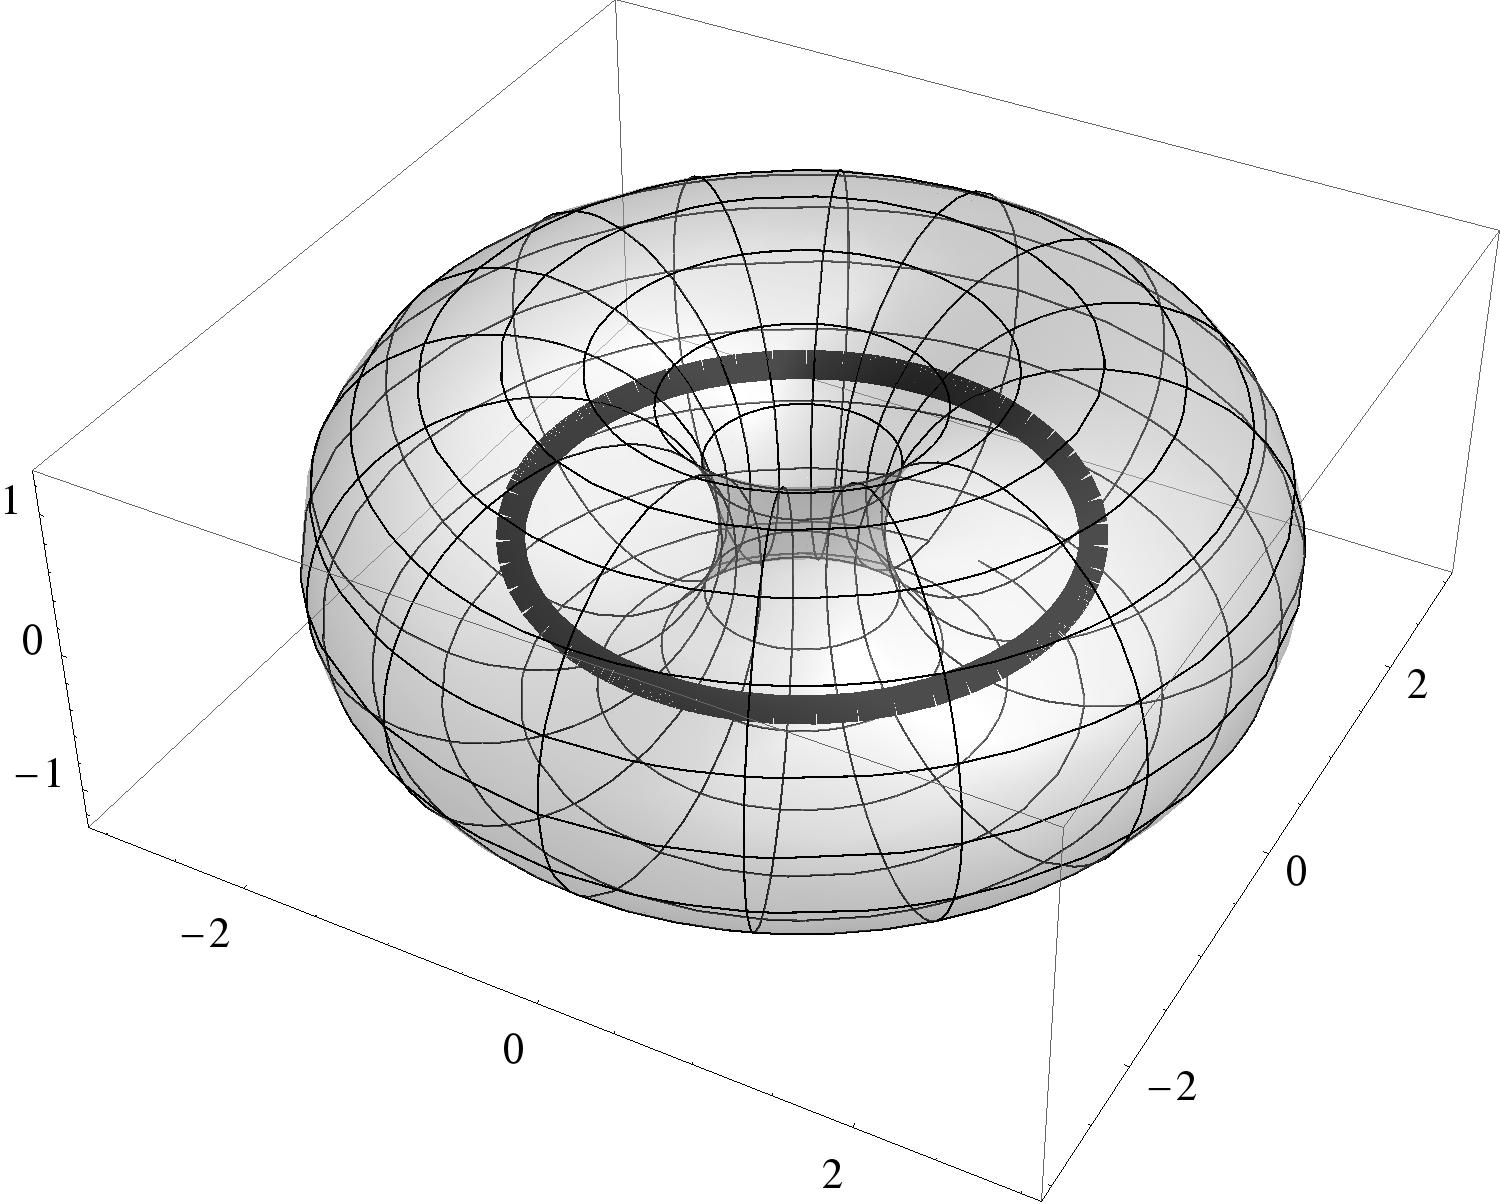
\includegraphics{transdonut.jpg}
    \end{image}
    Give a formula for a vector-valued function $\vec{p}(\theta)$ that will
    draw a circle in the $(x,y)$-plane, centered at the origin, of radius
    $R$, as $\theta$ runs from $0$ to $2\pi$.
    \[
    \vec{p}(\theta) = \vector{\answer[given]{R\cos(\theta)},\answer[given]{R\sin(\theta)},\answer{0}}
    \]
    Compute $\utan(\theta)$, the function that will give the unit tangent
    vector for any value of $\theta$. \textbf{Simplify your answer.}
    \[
    \utan(\theta) = \vector{\answer[given]{-\sin(\theta)},\answer[given]{\cos(\theta)},\answer[given]{0}}
    \]
    Compute $\unormal(\theta)$, the function that will give the principal
    unit normal vector for any value of $\theta$. \textbf{Simplify your answer.}
    \[
    \unormal(\theta) =\vector{\answer[given]{-\cos(\theta)},\answer[given]{-\sin(\theta)},\answer[given]{0}}
    \]
    Compute $\ubinormal(\theta)$, the function that will give the 
    unit binormal vector for any value of $\theta$. \textbf{Simplify your answer.}
    \begin{align*}
      \ubinormal(\theta) &= \utan(\theta)\cross\unormal(\theta)\\
      &=\vector{\answer[given]{0},\answer[given]{0},\answer[given]{1}}
    \end{align*}
    Now if we put these together we can write our torus as $\vec{T}(\theta,\phi)$
    \[
    \vec{T}(\theta,\phi) = \vec{p}(\theta) + \answer[given]{r}\cdot \unormal(\theta)\cos(\answer[given]{\phi}) + \answer[given]{r}\cdot \ubinormal(\theta)\sin(\answer[given]{\phi})
    \]
    Simplifying and writing the components of this formula out we see:
    \begin{align*}
      x(\theta,\phi) &= \answer[given]{(R - r\cdot \cos(\phi))\cos(\theta)}\\
      y(\theta,\phi) &= \answer[given]{(R - r\cdot \cos(\phi))\sin(\theta)}\\
      z(\theta,\phi) &= \answer[given]{r\cdot \sin(\phi)}
    \end{align*}
    And done. We've given a parametric formula for a torus.
  \end{explanation}
\end{example}

\begin{question}
  If you're paying attention, you may notice that we now have a very
  similar formula to the one given above, except that we have some
  minus signs where before we had plus signs. What happened here?
  \begin{prompt}
    \begin{multipleChoice}
      \choice{We made a mistake in our work in the example above.}
      \choice{We lied to you when we give the initial parametric formula for the torus.}
      \choice{We just broke math.}
      \choice[correct]{Everybody wins. Both formulas draw a torus.}
    \end{multipleChoice}
    \begin{feedback}[correct]
      Both formulas are correct, the first one we gave was derived
      using ``outward'' pointing normal vectors. The second one we
      gave was derived using ``inward'' pointing normal vectors.
    \end{feedback}
  \end{prompt}
\end{question}


\end{document}
